\documentclass{beamer}
\usepackage[french]{babel}
\usepackage[utf8]{inputenc}
\usepackage{graphicx}
%pour les tableaux
\usepackage{colortbl}
\usepackage{lmodern}
\usepackage{amsmath}
\usepackage{background}
\usepackage{tikz}

%Pour les fontes
\usefonttheme{serif}
\usepackage[T1]{fontenc}

\usepackage[absolute,showboxes,overlay]{textpos}
%\TPshowboxestrue % commenter une fois fini
\TPshowboxesfalse % décommenter pour faire disparaitre les boites
\textblockorigin{0mm}{0mm} % origine des positions

%Thème Warsaw (qui a trop la classe)
\useinnertheme[shadow=true]{rounded}
\useoutertheme{shadow}
\usecolortheme{orchid}
\usecolortheme{whale}

\setbeamercolor{rouge}{fg=red!80!black}
\setbeamercolor{footlinecolor}{fg=white,bg=black}
\setbeamercolor{footlinecolor2}{fg=white,bg=blue}

\setbeamertemplate{headline}{}

\setbeamertemplate{footline}{
	\leavevmode%
	\hbox{\hspace*{0.0cm}%
	\begin{beamercolorbox}[wd=.4\paperwidth,ht=2.25ex,dp=1ex,center]{section in head/foot}
	%\begin{beamercolorbox}[wd=.2\paperwidth,ht=2.25ex,dp=1ex,center]{author in head/foot}%
		\usebeamerfont{author in head/foot}\insertshortauthor%~~(\insertshortinstitute)
	\end{beamercolorbox}%
	\begin{beamercolorbox}[wd=.4\paperwidth,ht=2.25ex,dp=1ex,center]{section in head/foot}%
		\usebeamerfont{section in head/foot}\insertshorttitle
	\end{beamercolorbox}%
	\begin{beamercolorbox}[wd=.2\paperwidth,ht=2.25ex,dp=1ex,right]{section in head/foot}%
	%	\usebeamerfont{section in head/foot}\insertshortdate{}\hspace*{2em}
		\insertframenumber{}\hspace*{2ex}
		%\inserttotalframenumber
	\end{beamercolorbox}%
	}%
	\vskip0pt%
}

%ce sont les barres latérales, mais on en a pas besoin
%\setbeamersize{sidebar right width=0.0cm}
%\setbeamersize{sidebar left width=0.0cm}
%marges qui pourissent l'existence pour les alignements
\setbeamersize{text margin left=0.1cm}
\setbeamersize{text margin right=0.1cm}

\setbeamertemplate{navigation symbols}{
	\insertslidenavigationsymbol
%	\insertframenavigationsymbol
%	\insertsubsectionnavigationsymbol
%	\insertsectionnavigationsymbol
%	\insertdocnavigationsymbol
%	\insertbackfindforwardnavigationsymbol
}

\newenvironment<>{monblock}[2][\linewidth]{%
	\begin{center}%
	\begin{minipage}{#1}%
	\begin{actionenv}#3%
	\def\insertblocktitle{#2}%
	\par%
	\usebeamertemplate{block begin}
}{\par%
	\usebeamertemplate{block end}%
	\end{actionenv}%
	\end{minipage}%
	\end{center}%
}

\title[ ]{L'archivage de données}

\author{Pierre Aubert, Salim Nahi, Puchen Liu}

\begin{document}

\pgfdeclareimage[height=96mm,width=128mm]{bgTitle}{../images/happy_birthday_fraterchaos_by_jim373-d5vv1u7.jpg}

\setbeamertemplate{background}{\pgfuseimage{bgTitle}}
\frame{
	%\maketitle
	\begin{center}
		\begin{Huge}
			\color{white}
			\setbeamerfont{serif}{shape=\itshape,family=\rmfamily}
			\textbf{Projet CPA \\ Vectorisation de boucle}
		\end{Huge}
		\\
		\vspace{1cm}
		\begin{Large}
			\color{white}
			\textbf{Pierre Aubert, Salim Nahi, Puchen Liu}
		\end{Large}
	\end{center}
}

\setbeamertemplate{background}{}

\frame{
	\frametitle{Introduction}
	
	
}

\frame{
	\frametitle{La librairie d'analyse}
	\begin{monblock}[0.8\textwidth]{Les choses à analyser}
		\begin{itemize}
			\item Lecture après lecture
			\item Lecture après écriture
			\item Écriture après lecture
			\item Écriture après écriture
		\end{itemize}
	\end{monblock}
}

\frame{
	\frametitle{Le plugin}
	\begin{monblock}[0.8\textwidth]{Les choses à analyser}
		\begin{itemize}
			\item Analyse des boucles les plus profondes
			\item Insertion d'appels de fonction à la librairie
		\end{itemize}
	\end{monblock}
}

\frame{
	\frametitle{Le plugin}
	\begin{center}
		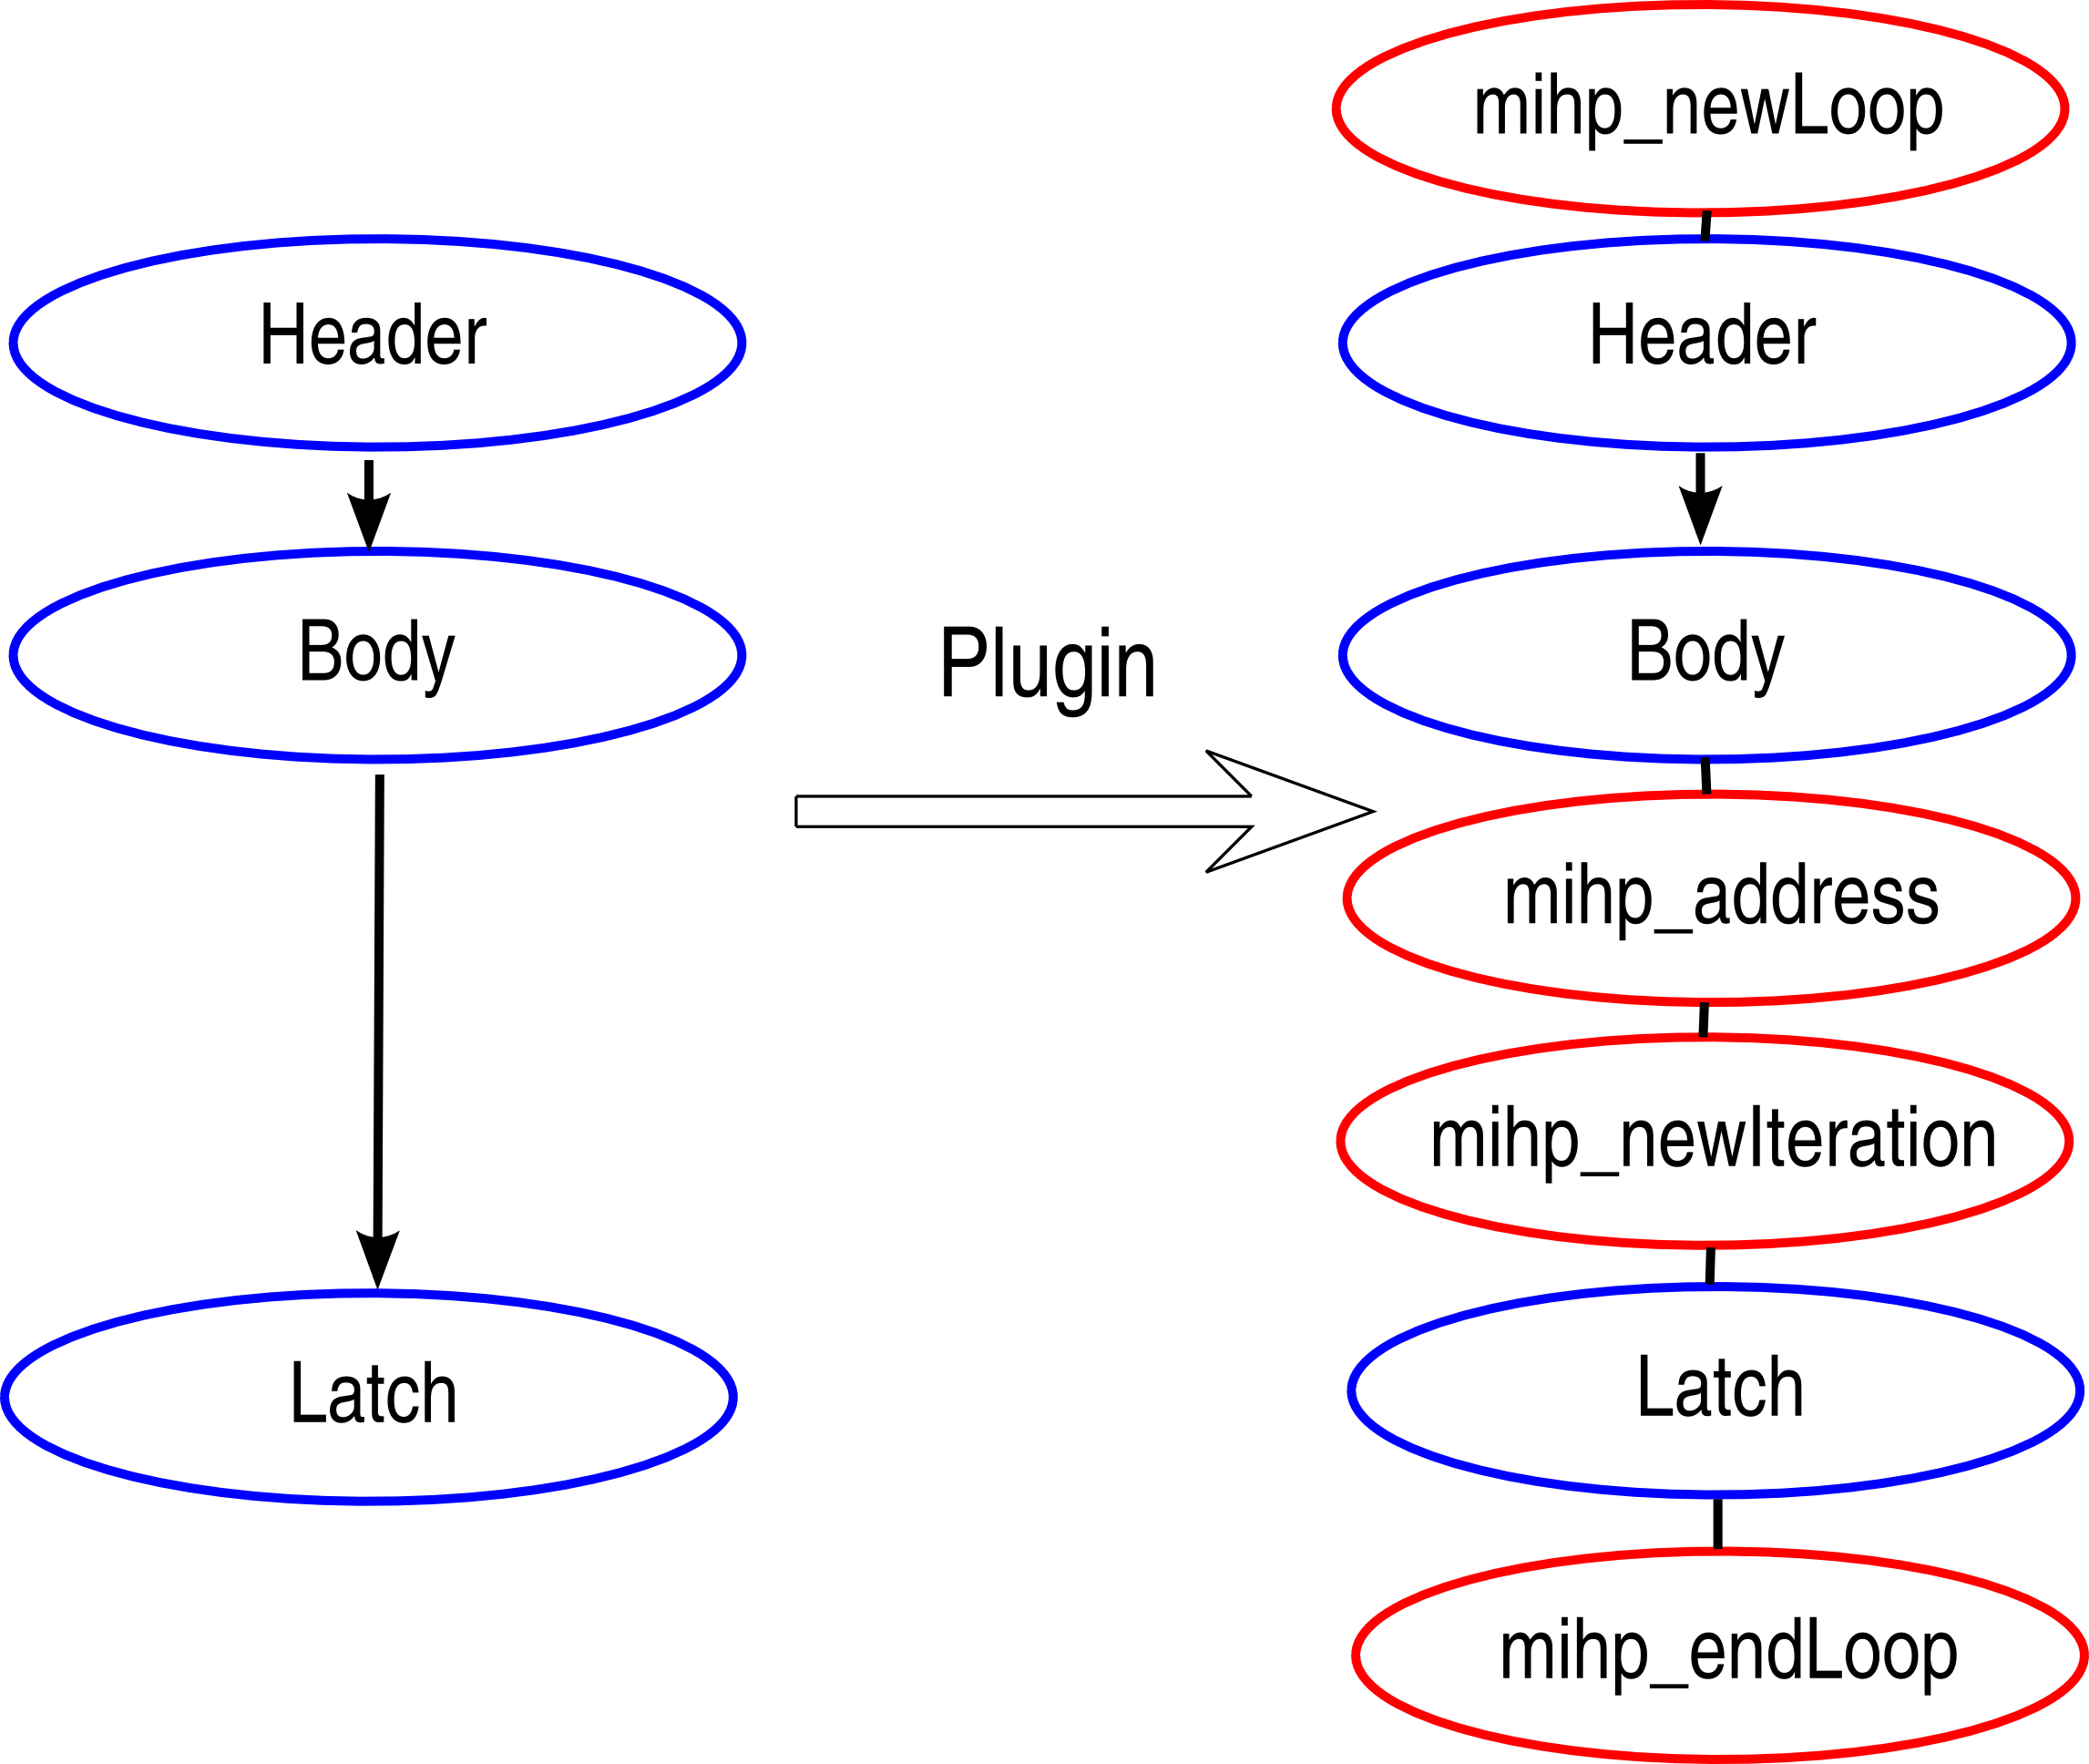
\includegraphics[scale=0.5]{../images/pluginInsertionFonctionAvant.png}
	\end{center}
}

\frame{
	%\maketitle
	\begin{center}
		\begin{Huge}
			\setbeamerfont{serif}{shape=\itshape,family=\rmfamily}
			\textbf{Merci de votre \\ attention}
		\end{Huge}
	\end{center}
}

\setbeamertemplate{background}{}
%\setbeamertemplate{background}[vertical shading][top=structure.fg!05,bottom=structure.fg!90]
%\setbeamertemplate{background}{}

\end{document}



